\chapter{Van grondstof tot recycling}\label{ch:g5:raw-materials-and-recycling}

Een leeg blikje verdwijnt in een recyclingbak. Een vrachtwagen brengt
het naar een sorteercentrum, een machine perst het samen met duizenden
andere tot een blok, een oven smelt de blokken, en een paar weken later
ligt het metaal als nieuw blikje weer in de winkel. Waar kwam het metaal
oorspronkelijk vandaan, en waarom is het de moeite waard om oude blikjes
om te smelten in plaats van nieuw metaal te maken?

\begin{recall}
Een voorwerp is een ding dat we kunnen zien en aanraken; het materiaal
is waar het van gemaakt is --- hout, metaal, glas, plastic, papier,
textiel, steen (\cref{ch:g1:materials-around-us}). Bij een \omterm{def:g5:irreversible-changes:chemical-change}{chemische
verandering} ontstaan nieuwe stoffen en is er geen eenvoudige weg terug
(\cref{ch:g5:irreversible-changes}).
\end{recall}

\section{Natuurlijke en vervaardigde materialen}

\begin{definition}[Natuurlijke en vervaardigde materialen]\label{def:g5:raw-materials-and-recycling:natural-material}
Een \emph{natuurlijk materiaal}\index{natuurlijk materiaal} gebruik je
ongeveer zoals je het in de natuur vindt, alleen gezaagd of in vorm
gebracht: hout, steen, katoen, wol, leer. Een \emph{vervaardigd
materiaal}\index{vervaardigd materiaal} maken mensen uit stoffen uit de
natuur, door ze te veranderen, vaak met warmte en \omterm{def:g5:irreversible-changes:chemical-change}{chemische
veranderingen}: glas, staal, aluminium, plastic, papier, beton.
\end{definition}

\begin{example}[Twee tafels]\label{ex:g5:raw-materials-and-recycling:tables}
Een tafel van eikenhouten planken is van een \omterm{def:g5:raw-materials-and-recycling:natural-material}{natuurlijk materiaal}
gemaakt: het hout is alleen gezaagd, geschaafd en gelijmd. Een tafel met
een glazen blad en stalen poten is van \omterm{def:g5:raw-materials-and-recycling:natural-material}{vervaardigde materialen} gemaakt:
glas en staal vind je niet zomaar in de natuur.
\end{example}

\section{Grondstoffen}

\begin{definition}[Grondstof en erts]\label{def:g5:raw-materials-and-recycling:raw-material}
Een \emph{grondstof}\index{grondstof} is een stof die uit de natuur
gehaald wordt om er materialen en voorwerpen van te maken: bomen, zand,
gesteenten, ruwe aardolie, katoen, wol. Een gesteente waaruit een metaal
gewonnen wordt, heet een \emph{erts}\index{erts}.
\end{definition}

\begin{example}[Waar materialen vandaan komen]\label{ex:g5:raw-materials-and-recycling:from}
\begin{itemize}
  \item hout en papier komen van bomen;
  \item glas komt van zand, heel sterk verhit met soda en kalksteen;
  \item ijzer en staal komen van ijzererts, een roodachtig gesteente;
  \item aluminium komt van bauxiet, een ander \omterm{def:g5:raw-materials-and-recycling:raw-material}{erts};
  \item de meeste soorten plastic komen van ruwe aardolie, die uit de
        grond wordt opgepompt;
  \item katoen komt van een plant, wol van schapen.
\end{itemize}
\end{example}

\begin{omfigure}
\begin{minipage}[b]{0.48\linewidth}\centering
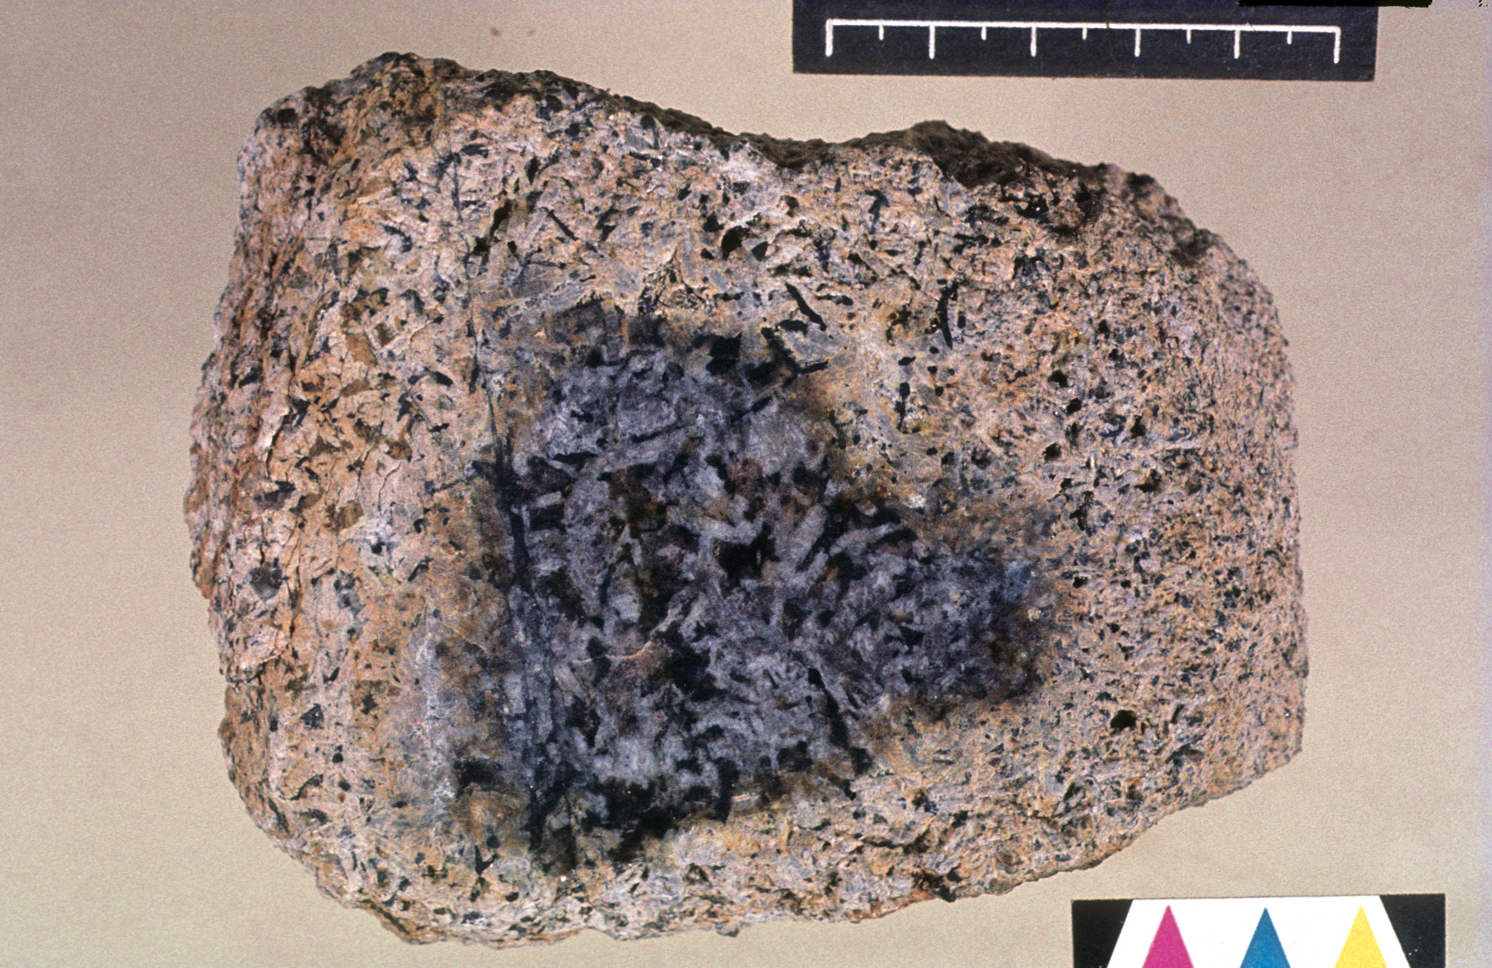
\includegraphics[width=\linewidth,height=4.6cm,keepaspectratio]{images/book1/bauxite.jpg}

{\small Bauxiet, het \omterm{def:g5:raw-materials-and-recycling:raw-material}{erts} van aluminium, rond een kern van onverweerd
gesteente. Foto: Werner Schellmann, CC BY-SA 2.5.}
\end{minipage}\hfill
\begin{minipage}[b]{0.48\linewidth}\centering
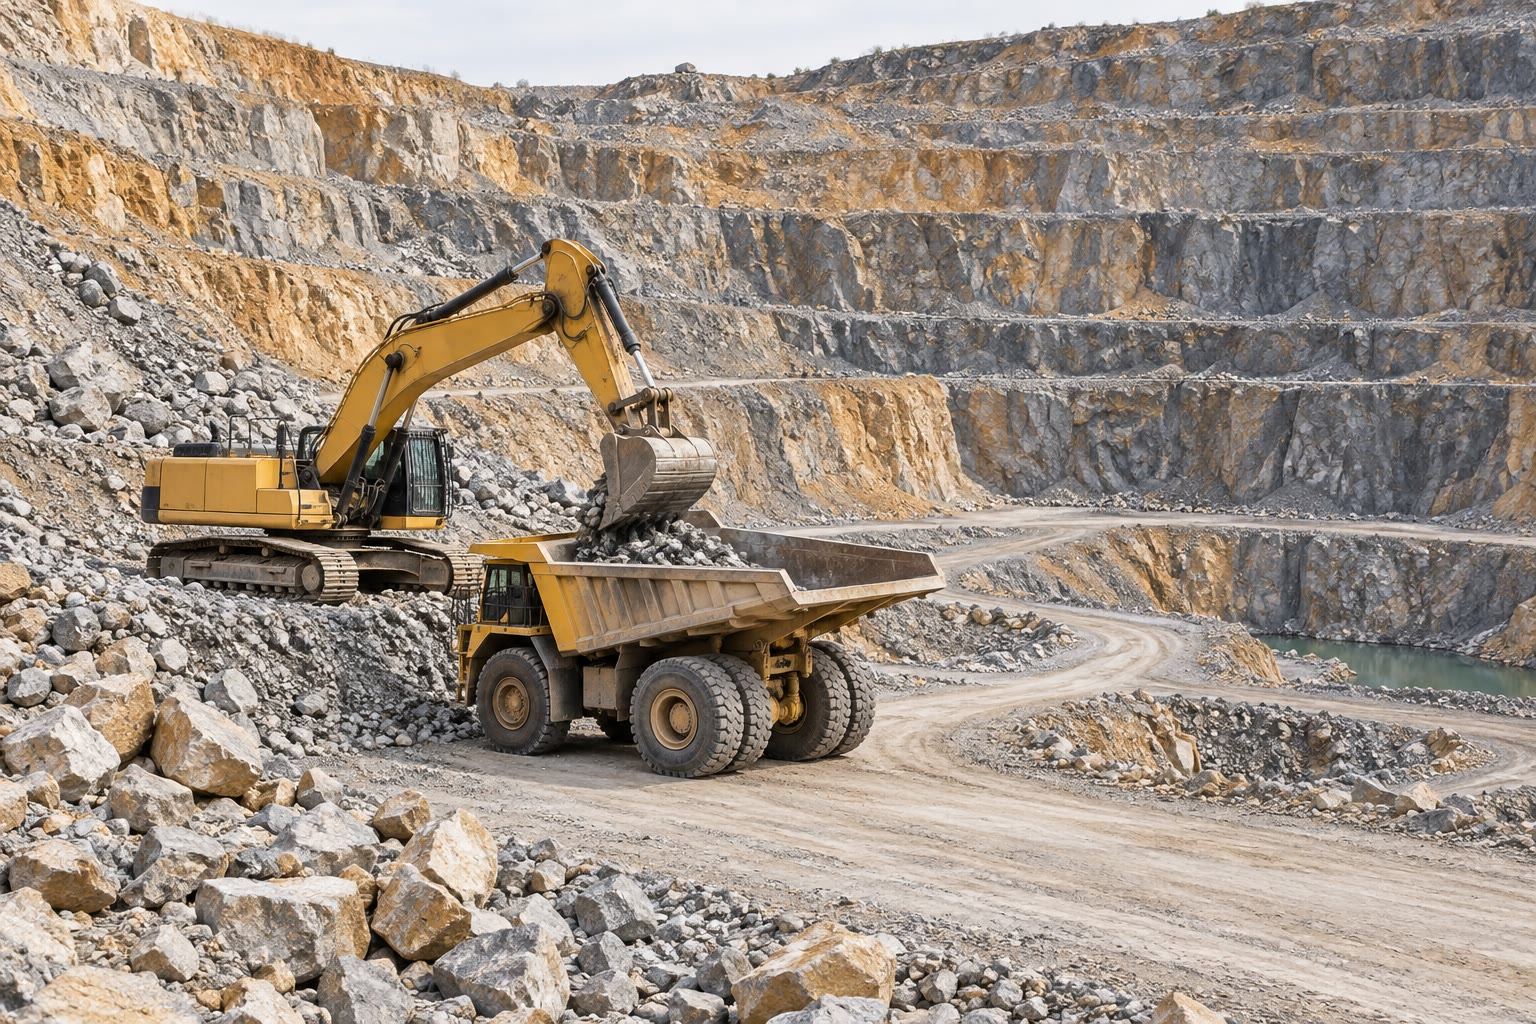
\includegraphics[width=\linewidth,height=4.6cm,keepaspectratio]{images/book1/ai/g5-quarry.jpg}

{\small Een steengroeve: er wordt gesteente uitgegraven om als \omterm{def:g5:raw-materials-and-recycling:raw-material}{grondstof}
te gebruiken.}
\end{minipage}
\end{omfigure}

\begin{omfigure}
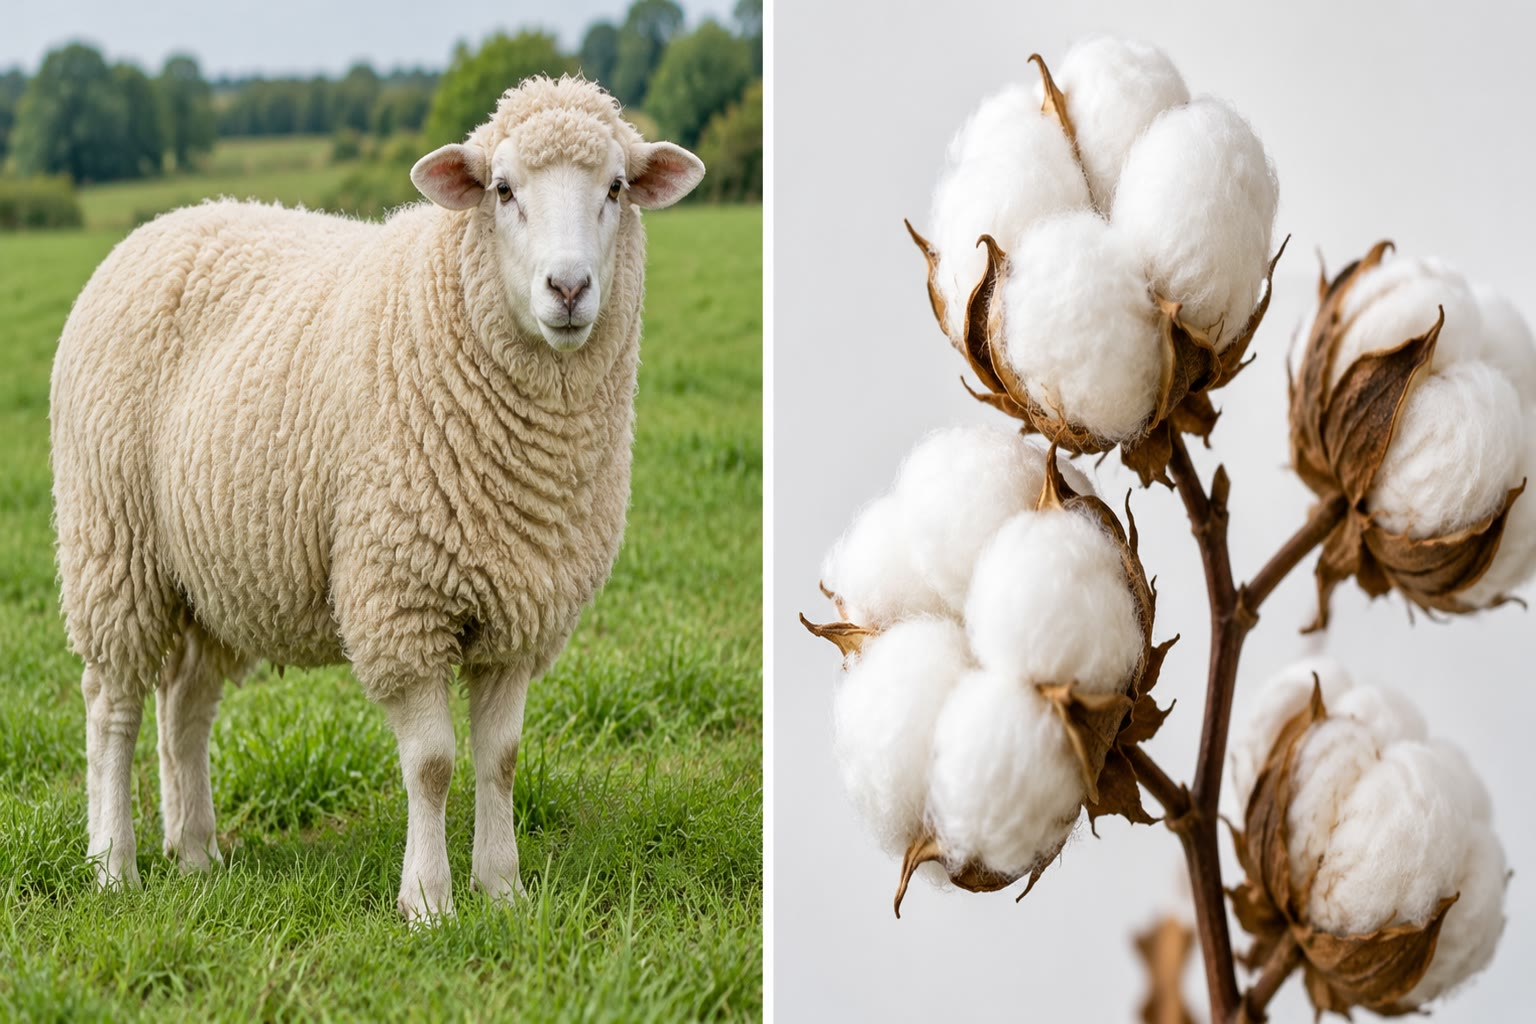
\includegraphics[width=0.6\linewidth]{images/book1/ai/g5-sheep-cotton.jpg}

{\small Natuurlijke \omterm{def:g5:raw-materials-and-recycling:raw-material}{grondstoffen} van levende wezens: wol van schapen,
katoen van de katoenplant.}
\end{omfigure}

\section{Van grondstof tot voorwerp}

\begin{proposition}[Bij het maken van een materiaal verandert de grondstof]\label{prop:g5:raw-materials-and-recycling:change}
Om van een \omterm{def:g5:raw-materials-and-recycling:raw-material}{grondstof} een \omterm{def:g5:raw-materials-and-recycling:natural-material}{vervaardigd materiaal} te maken, is energie
nodig --- meestal de warmte van een oven --- en meestal ook \omterm{def:g5:irreversible-changes:chemical-change}{chemische
veranderingen}: zand wordt glas, \omterm{def:g5:raw-materials-and-recycling:raw-material}{erts} wordt metaal, aardolie wordt
plastic. Die veranderingen kun je niet zomaar terugdraaien: glas wordt
nooit meer zand.
\end{proposition}

\begin{example}[Het leven van een glazen fles]\label{ex:g5:raw-materials-and-recycling:bottle}
Zand, soda en gemalen kalksteen worden samen in een oven verhit tot ze
smelten tot glas. Het hete glas wordt in de vorm van een fles geblazen.
De fles wordt gevuld, verkocht en leeggemaakt. In de glasbak gegooid,
wordt ze in kleine stukjes gebroken, opnieuw gesmolten en tot een nieuwe
fles geblazen: het glas wordt telkens opnieuw gebruikt.
\end{example}

\begin{omfigure}
\begin{tikzpicture}[font=\small,
    box/.style={draw=omDef, fill=omDef!6, rounded corners=2pt, align=center,
      minimum height=0.95cm, text width=2.4cm}]
  \node[box] (r) at (0,2.6) {grondstof\\ (zand, erts, olie)};
  \node[box] (m) at (4.0,2.6) {het materiaal\\ maken};
  \node[box] (o) at (8.0,2.6) {voorwerp,\\ gebruikt};
  \node[box] (w) at (8.0,0) {afval};
  \node[box, draw=omProp, fill=omProp!8] (s) at (4.0,0) {sorteren en\\ recyclen};
  \draw[->, thick, omDef] (r) -- (m);
  \draw[->, thick, omDef] (m) -- (o);
  \draw[->, thick, omDef] (o) -- (w);
  \draw[->, thick, omProp] (w) -- (s);
  \draw[->, thick, omProp] (s) -- (m) node[midway, left, align=right, text=black]
    {opnieuw gebruikt\\ in plaats van nieuwe\\ grondstof};
  \draw[->, thick, black!45, dashed] (w.east) -- ++(1.4,0) node[right, align=left,
    text=black] {weggegooid:\\ stortplaats};
\end{tikzpicture}

{\small Het leven van een materiaal. De oranje lus is \omterm{def:g5:raw-materials-and-recycling:recycling}{recycling}: het
materiaal van een oud voorwerp vervangt nieuwe \omterm{def:g5:raw-materials-and-recycling:raw-material}{grondstof}.}
\end{omfigure}

\section{Sorteren en recyclen}

\begin{definition}[Recycling]\label{def:g5:raw-materials-and-recycling:recycling}
\emph{Recycling}\index{recycling} is gebruikte voorwerpen inzamelen en
hun materiaal zo behandelen dat er nieuwe voorwerpen van gemaakt kunnen
worden, in plaats van het weg te gooien.
\end{definition}

\begin{proposition}[Waarom recyclen]\label{prop:g5:raw-materials-and-recycling:why}
% ledger: al:energy-primary, al:energy-recycled (8.3 / 186 = about 1/22)
\omterm{def:g5:raw-materials-and-recycling:recycling}{Recycling} bespaart \omterm{def:g5:raw-materials-and-recycling:raw-material}{grondstoffen}, die dan niet uit de grond gehaald
hoeven te worden, en het bespaart vaak energie. Aluminium maken uit oude
blikjes kost maar ongeveer een twintigste van de energie die nodig is om
het uit bauxiet te maken. Het betekent ook minder afval op de
stortplaatsen.
\end{proposition}

\begin{method}[Afval sorteren voor recycling]\label{met:g5:raw-materials-and-recycling:sort}
\omterm{def:g5:raw-materials-and-recycling:recycling}{Recycling} begint met sorteren, overal waar afval wordt weggegooid:
\begin{enumerate}
  \item glazen flessen en potten in één bak;
  \item metalen blikjes, papier en karton, en plastic flessen in de
        bakken die de gemeente daarvoor neerzet (de kleuren van de bakken
        verschillen van plaats tot plaats);
  \item wat niet gerecycled kan worden bij het restafval.
\end{enumerate}
Elk materiaal wordt op zijn eigen manier gerecycled, dus in een bak mag
alleen het materiaal waar hij voor bedoeld is.
\end{method}

\begin{omfigure}
\begin{tikzpicture}[font=\small]
  \foreach \k/\t/\bc in {0/glas/green!50!black, 1/{metalen blikjes}/gray,
                        2/{papier en karton}/omDef, 3/{plastic flessen}/orange!80!black} {
    \begin{scope}[xshift=\k*3.4cm]
      \fill[\bc!18, draw=\bc, line width=0.8pt] (-1,0) -- (1,0) -- (1.15,2.0)
        -- (-1.15,2.0) -- cycle;
      \fill[\bc!45, draw=\bc] (-1.25,2.0) rectangle (1.25,2.3);
      \node[anchor=north, align=center] at (0,-0.15) {\t};
    \end{scope}
  }
  % glass: a bottle
  \fill[green!40!black!60] (-0.2,0.3) rectangle (0.2,1.2);
  \fill[green!40!black!60] (-0.07,1.2) rectangle (0.07,1.6);
  % metal: a can
  \begin{scope}[xshift=3.4cm]
    \fill[black!25, draw=black!55] (-0.3,0.3) rectangle (0.3,1.3);
  \end{scope}
  % paper: a box and a sheet
  \begin{scope}[xshift=6.8cm]
    \fill[brown!25, draw=brown!60] (-0.6,0.3) rectangle (0.1,1.0);
    \fill[white, draw=black!40] (0.2,0.3) rectangle (0.65,1.3);
  \end{scope}
  % plastic: a bottle
  \begin{scope}[xshift=10.2cm]
    \fill[cyan!20, draw=cyan!50!black] (-0.25,0.3) rectangle (0.25,1.3);
    \fill[cyan!20, draw=cyan!50!black] (-0.1,1.3) rectangle (0.1,1.6);
  \end{scope}
\end{tikzpicture}

{\small Vier sorteerbakken, één per materiaal. (De kleuren van echte
bakken verschillen van gemeente tot gemeente.)}
\end{omfigure}

\begin{omfigure}
\begin{minipage}[t]{0.48\linewidth}\centering
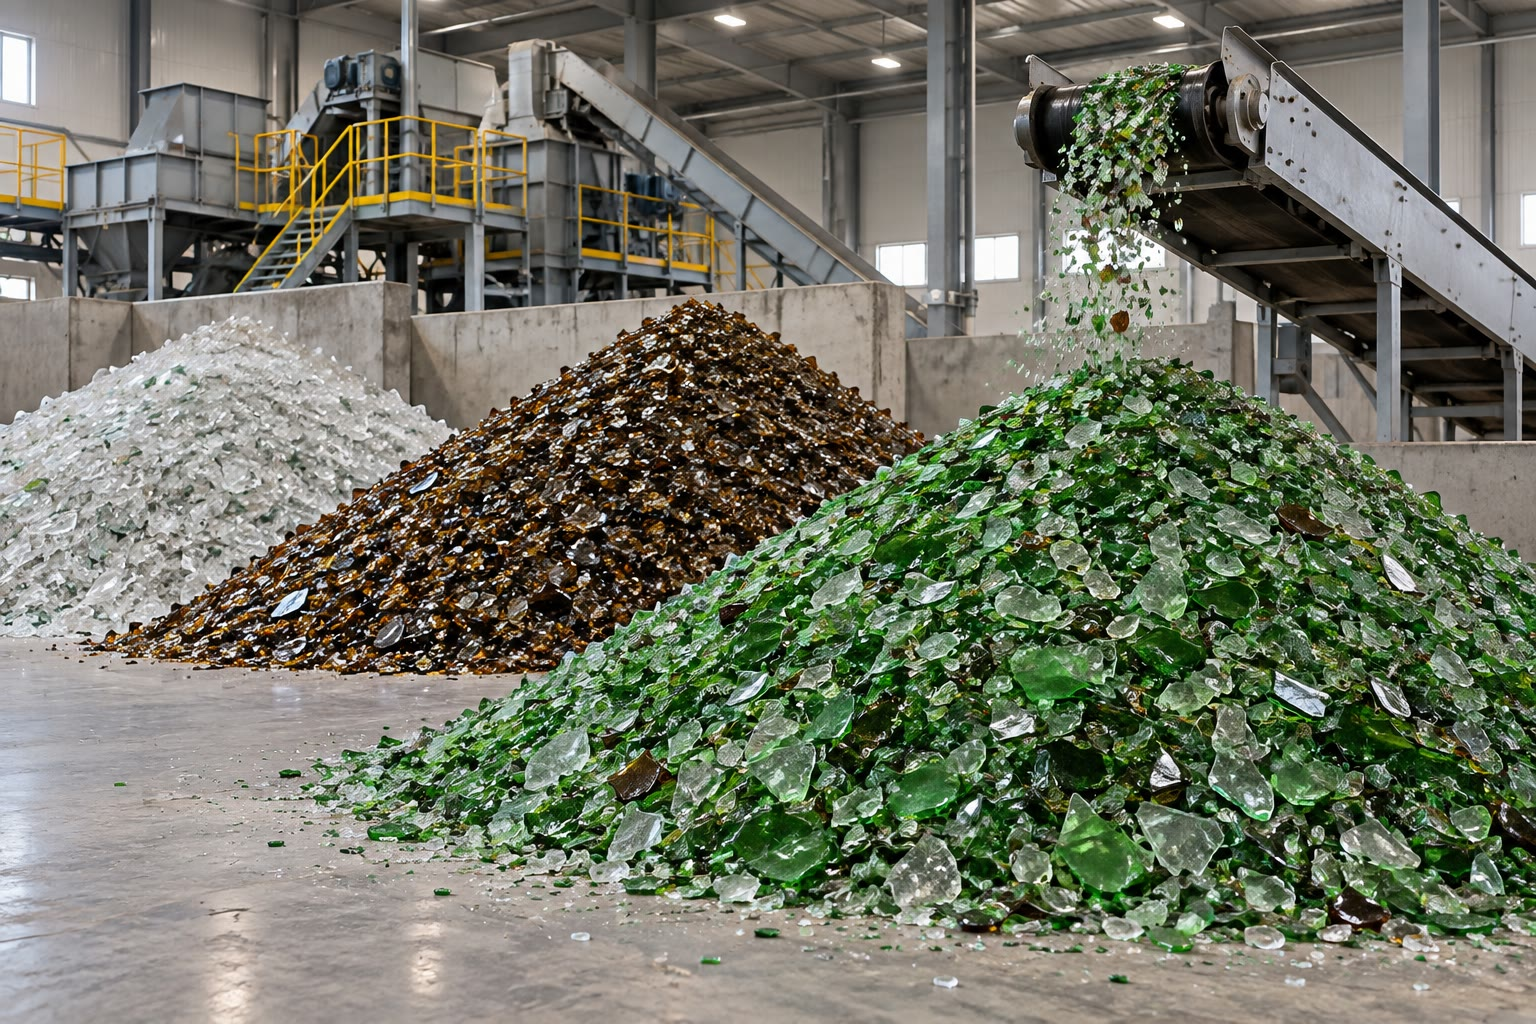
\includegraphics[width=\linewidth,height=4.6cm,keepaspectratio]{images/book1/ai/g5-glass-cullet.jpg}

{\small Gebroken glas in een recyclingfabriek, klaar om gesmolten te
worden.}
\end{minipage}\hfill
\begin{minipage}[t]{0.48\linewidth}\centering
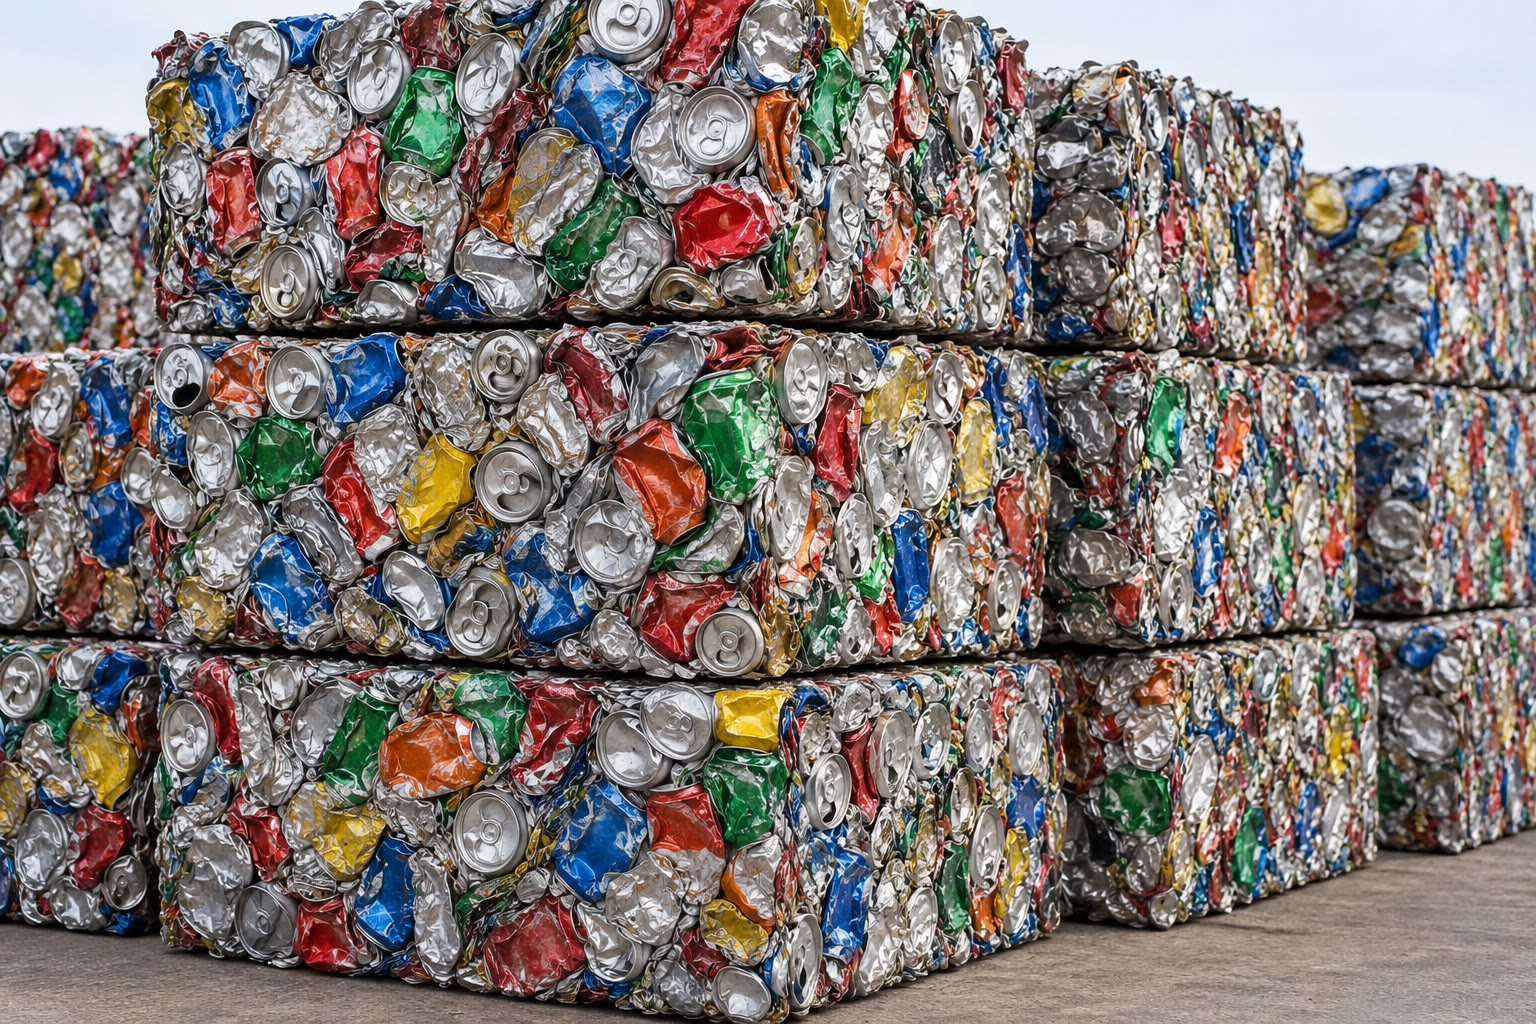
\includegraphics[width=\linewidth,height=4.6cm,keepaspectratio]{images/book1/ai/g5-can-bales.jpg}

{\small Balen geperste aluminium blikjes.}
\end{minipage}
\end{omfigure}

\section{Afval en hulpbronnen}

\begin{definition}[Hulpbron]\label{def:g5:raw-materials-and-recycling:resource}
Een \emph{hulpbron}\index{hulpbron} is alles wat mensen uit de natuur
halen en gebruiken: water, hout, ertsen, olie, zand. Een
\emph{hernieuwbare hulpbron}\index{hernieuwbare hulpbron} groeit vanzelf
weer aan of komt vanzelf terug binnen een mensenleven, zoals hout uit
een bos dat opnieuw wordt aangeplant, of wol van schapen. Ertsen en ruwe
aardolie zijn niet hernieuwbaar: als ze eenmaal uitgegraven en gebruikt
zijn, zijn ze op.
\end{definition}

\begin{proposition}[Minderen, hergebruiken, recyclen]\label{prop:g5:raw-materials-and-recycling:three}
Om \omterm{def:g5:raw-materials-and-recycling:resource}{hulpbronnen} langer te laten meegaan, kunnen mensen, in deze
volgorde:
\begin{enumerate}
  \item \textbf{minderen}: minder voorwerpen gebruiken, bijvoorbeeld
        minder verpakkingen;
  \item \textbf{hergebruiken}: hetzelfde voorwerp opnieuw gebruiken,
        zoals een glazen pot die je opnieuw vult of een tas die je mee
        terugneemt naar de winkel;
  \item \textbf{recyclen}: van het materiaal een nieuw voorwerp maken.
\end{enumerate}
Recyclen komt als laatste, omdat er nog altijd energie en machines voor
nodig zijn; het beste afval is afval dat nooit gemaakt wordt.
\end{proposition}

\section{Oefeningen}

\begin{exercise}[$\star$]\label{exo:g5:raw-materials-and-recycling:1}
Natuurlijk of vervaardigd? Hout, glas, wol, staal, plastic, steen.
\end{exercise}

\begin{exercise}[$\star$]\label{exo:g5:raw-materials-and-recycling:2}
Geef de \omterm{def:g5:raw-materials-and-recycling:raw-material}{grondstof} van: een vel papier, een glazen pot, een katoenen
T-shirt, een plastic fles.
\end{exercise}

\begin{exercise}[$\star$]\label{exo:g5:raw-materials-and-recycling:3}
Wat is een \omterm{def:g5:raw-materials-and-recycling:raw-material}{erts}? Noem het \omterm{def:g5:raw-materials-and-recycling:raw-material}{erts} van aluminium.
\end{exercise}

\begin{exercise}[$\star$]\label{exo:g5:raw-materials-and-recycling:4}
In welke bak gooi je: een lege jampot, een krant, een blikje, een
plastic waterfles?
\end{exercise}

\begin{exercise}[$\star$]\label{exo:g5:raw-materials-and-recycling:5}
Kijk naar de figuur van het leven van een materiaal. Wat vervangt de
oranje lus?
\end{exercise}

\begin{exercise}[$\star$]\label{exo:g5:raw-materials-and-recycling:6}
Hernieuwbaar of niet: hout, ruwe aardolie, wol, ijzererts, katoen?
\end{exercise}

\begin{exercise}[$\star$]\label{exo:g5:raw-materials-and-recycling:7}
Waarom kun je glas niet weer zand laten worden door het af te koelen?
\end{exercise}

\begin{exercise}[$\star$]\label{exo:g5:raw-materials-and-recycling:8}
Geef een manier om te minderen, een manier om te hergebruiken en een
manier om te recyclen.
\end{exercise}

\begin{exercise}[$\star$]\label{exo:g5:raw-materials-and-recycling:9}
Waarom mag er in een glasbak alleen glas?
\end{exercise}

\begin{exercise}[$\star\star$]\label{exo:g5:raw-materials-and-recycling:10}
Aluminium maken uit oude blikjes kost ongeveer een twintigste van de
energie die nodig is om het uit bauxiet te maken. Een fabriek gebruikt
20 eenheden energie om een partij aluminium uit bauxiet te maken.
Ongeveer hoeveel eenheden zou ze gebruiken om dezelfde partij uit oude
blikjes te maken?
\end{exercise}

\begin{exercise}[$\star\star$]\label{exo:g5:raw-materials-and-recycling:11}
Waarom staat ``minderen'' vóór ``recyclen''?
\end{exercise}
